\chapter{Related Work and State of the Art}
\label{chapter:related work}

\section{Taxonomies for Classification of Occupations, Skills and Competences}

The collection of data about occupations, skills and competences from a variety of sources resulted in the creation of structured databases for occupational classification, the taxonomies~\cite{CHIARELLO2021121177}. 

This classification through these various taxonomies plays a crucial role in the modern labour market and educational landscape. They serve as structured frameworks to categorize and describe occupations and the skills required for them in a standardized way, facilitating communication, analysis, and planning across different sectors and geographical boundaries.

Nowadays, their importance is undeniable, so we highlight the following advantages~\cite{labour_market_info, world_eco_forum}:
\begin{itemize}
\item{Standardization and clarity - these taxonomies provide a common language for describing jobs and skills which is particularly important in a globalized economy where workers, employers, educators and long-life learners operate across different regions and countries. For example, if an individual completed a Bachelor’s degree in Portugal and a Master’s degree in France and, for some reason, wants to work in Germany, these taxonomies would help their German employer to understand which skills the individual possesses and recognize their higher education degrees.}
\item{Labour market analysis - They enable government agencies, economists, and researchers to analyze labour market trends, track occupational shifts, and predict future workforce needs. This information is vital for policy-making, especially in areas like employment, education, and immigration.}
\item{Career development and guidance - For individuals, these taxonomies offer valuable insights into the skills and qualifications required for various occupations, aiding in career planning and development. They are particularly useful for long-life learners who are looking to update their skills or change career paths.}
\item{Recruitment and human resource management - Enterprises utilize these taxonomies to define job roles, assess skill requirements, and align their workforce with organizational needs. This alignment is crucial for effective human resource management and strategic planning.}
\item{Educational planning and curriculum development - Education institutions use these taxonomies to align their curricula with the current and future needs of the labour market. This ensures that the skills and knowledge they impart are relevant and meet industry standards.}
\end{itemize}


In this section we’ll present some examples of taxonomies, focusing our attention on ESCO since it will be the matter of study of this thesis.

\subsection{ESCO}
\label{sec:esco}
Citing the European Commission’s ESCO website: “\ac{esco} is the European multilingual classification of Skills, Competences and Occupations. \ac{esco} works as a dictionary, describing, identifying and classifying professional occupations and skills relevant for the EU labour market,  education and training”~\cite{what_esco}. This taxonomy allows computational systems to use the three pillars of ESCO (occupations, skills and qualifications)~\cite{Fareri_2021} and the relationships between them to address different use cases, such as matching job seekers to jobs on the basis of their skills, suggesting training programmes to life-long learners, understanding which qualifications are demanded or often requested by employers for working in a specific occupation, etc.

\begin{figure}[H]
    \centering
    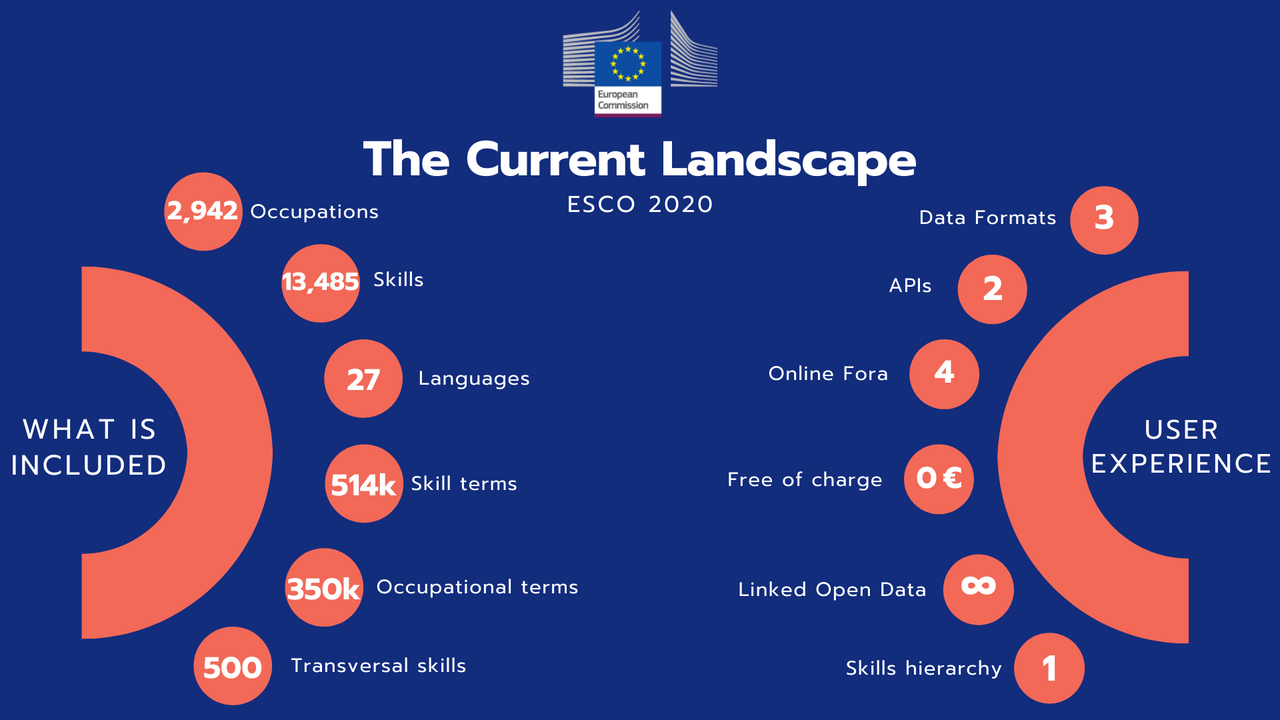
\includegraphics[width=15cm]{figs/ESCO_Landscape.png}
    \caption{\acs{esco}'s Landscape in September 2022 - currently the taxonomy contains information about 3,008 occupations and 13,890 skills~\cite{what_esco}}
    \label{fig:esco_landscape}
\end{figure}

People change jobs and employers more frequently than in the past, new skills are regularly needed while geographic and job mobility increases. Both employers and job seekers are turning more to digital methods for posting and applying for jobs, as well as for seeking and providing training opportunities. Companies and educational institutions need clear and updated information on skills and qualifications to better address skills gaps in education~\cite{esco_needed}.  

Therefore, the aim of \ac{esco} is to support job mobility across Europe and, consequently, achieve a more integrated and efficient labour market, by offering a “common language” on occupations and skills that can be used by different stakeholders on employment, education and training topics~\cite{what_esco}. 

\ac{esco}’s classification can be accessed through two types of APIs, a web-service API, available online, and a Local API which, as the name suggests, needs to be installed locally~\cite{esco_api}.

The \ac{esco} Web Services API is a web-based service that offers access to various versions of the \ac{esco} classification, encompassing functionalities that address most \ac{esco} business use cases. Featuring an easy-to-use web interface for linked data (disposed hierarchically), each concept is identified as an URI, making it a perfect setup for non-technical users. This service allows text search for Occupations, Skills \& Competences and Qualifications.

\begin{figure}[H]
    \centering
    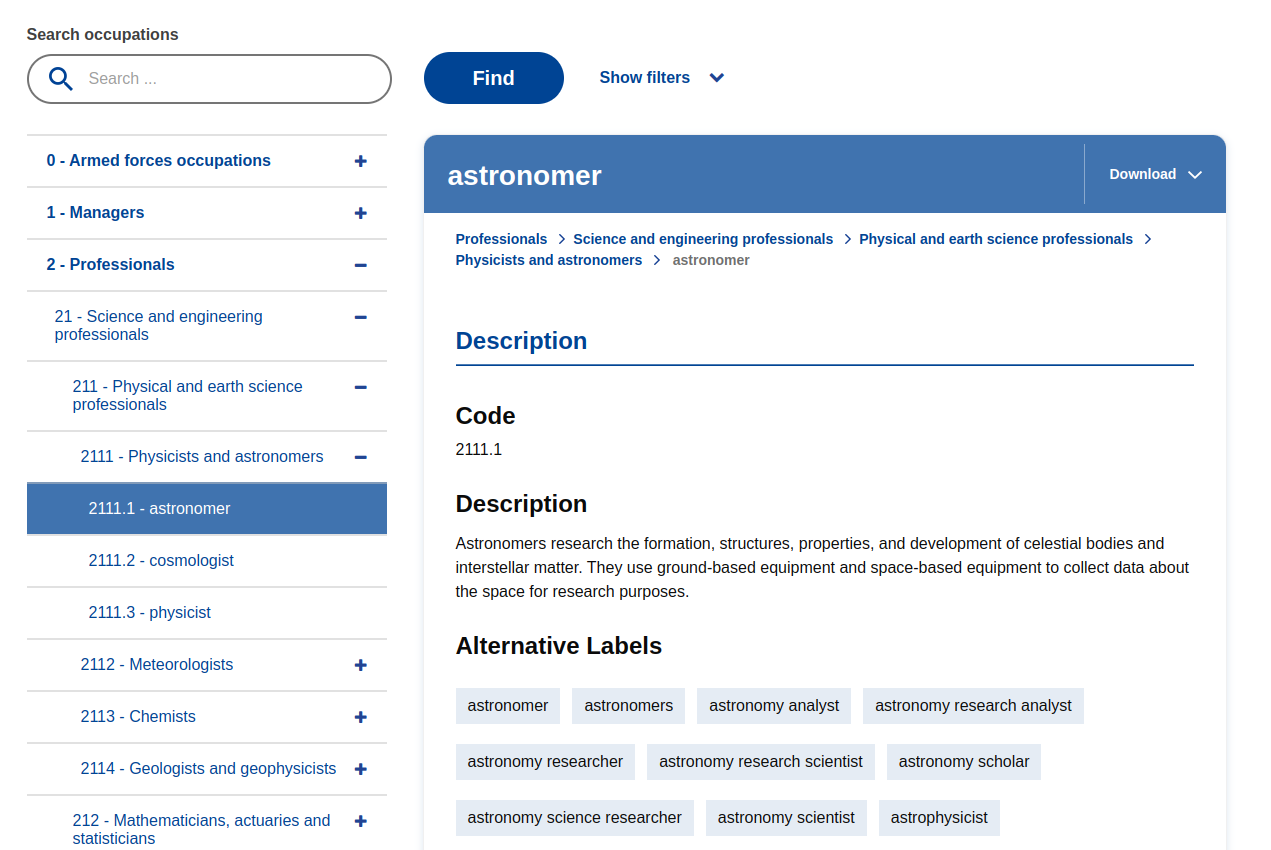
\includegraphics[width=15cm]{figs/esco_web_service.png}
    \caption{Example of an \acs{esco}'s Web Service page~\cite{astronomer}}
    \label{fig:esco_web_service}
\end{figure}

The \ac{esco} Local API is a downloadable version of the \ac{esco} API, which can be installed on a computer or server, providing local access to \ac{esco}’s information. Compared to the Web Services API, this local version assures increased performance and the independence from the availability of the service provided by the European Commission.

\subsection{ISCO}
The \ac{isco} is a globally recognized framework developed by the International Labour Organization (ILO) to categorize and organize occupations~\cite{isco}. Just like \ac{esco}, this taxonomy serves as a vital tool for labour market analysis, providing a standardized system for classifying jobs based on the skills, education, and duties involved. \ac{isco} is structured hierarchically, with major groups divided into sub-major groups, minor groups, and unit groups, each with different levels of detail and specificity. The two latest versions of \ac{isco} are ISCO-88 (dating from 1988) and ISCO-08 (dating from 2008)~\cite{esco_isco_relation}.
\ac{esco} was actually influenced and inspired by \ac{isco}, particularly in its approach to structuring occupations. \ac{esco} maps each occupation to an ISCO-08 code and uses ISCO-08 as a hierarchical structure for its occupations pillar, indicating a direct link and a level of compatibility and interoperability between the two systems~\cite{esco_isco}.

\begin{figure}[H]
    \centering
    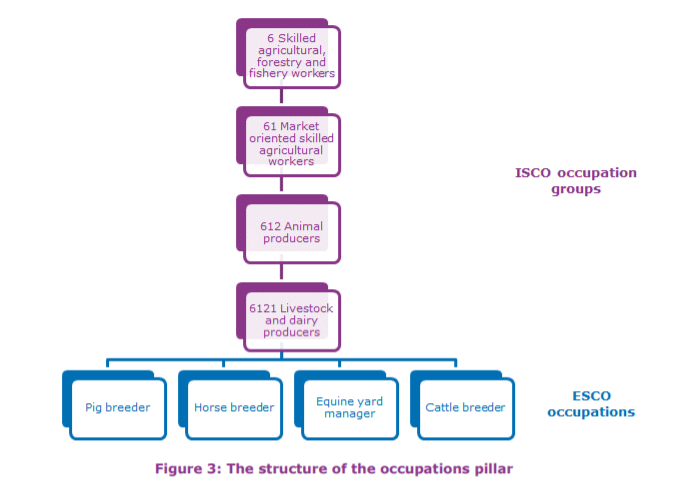
\includegraphics[width=15cm]{figs/esco_isco.png}
    \caption{Role of ISCO-08 in the hierarchical structure of the ESCO occupations pillar~\cite{esco_isco}}
    \label{fig:esco_isco}
\end{figure}


This alignment with ISCO-08 enables \ac{esco} to both:
\begin{itemize}
    \item maintain consistency with a globally recognized occupational classification system, ensuring harmonization with international standards.
    \item enhance its utility for the European labour market - facilitating comprehensive market analysis and mobility across borders.
\end{itemize}


\subsection{O*NET}
\ac{onet} is the American equivalent of \ac{esco}, developed under the sponsorship of the U.S. Department of Labor/Employment and Training Administration (USDOL/ETA)~\cite{esco_onet_crosswalk}, comprising occupations from the Standard Occupational Classification (SOC) system and their corresponding skills, knowledge, and abilities~\cite{Fareri_2021}.
Just like the above taxonomies, \ac{onet} aims to provide a comprehensive database of job characteristics and work skills that standardizes and categorizes the labour market, in this case, of the American panorama.

\begin{figure}[H]
    \centering
    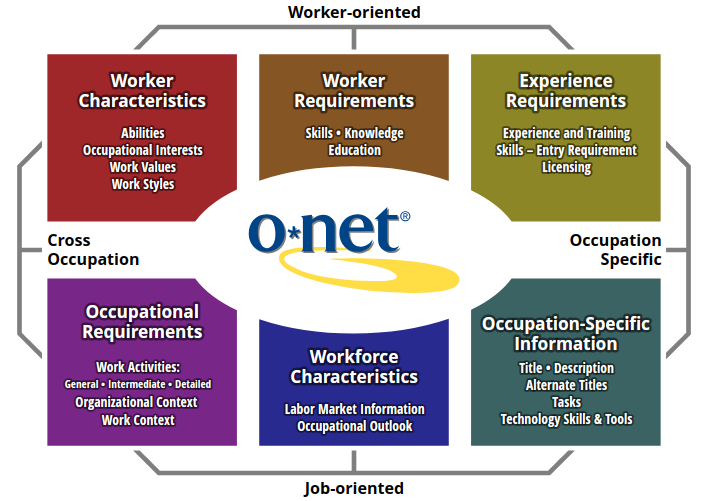
\includegraphics[width=15cm]{figs/onet_content_model.png}
    \caption{The O*NET® Content Model schematic representation~\cite{onet_content}}
    \label{fig:onet_content}
\end{figure}

The \ac{onet} Content Model~\cite{onet_content} serves as the structural foundation for the \ac{onet} database, outlining critical occupational information by integrating job-oriented and worker-oriented descriptors. Developed through job analysis research, it includes six domains that detail attributes and characteristics relevant both across occupations (cross-occupational descriptors) and within specific jobs (occupation-specific descriptors), facilitating a comprehensive understanding of various roles and worker qualities.

According to~\citeauthor{Fareri_2021}, when compared to \ac{esco}, this taxonomy lacks in the level of detail, as the latter possesses six times more skills and three times as many job profiles~\cite{Fareri_2021}.
Furthermore, there was a cooperation between the \ac{esco} Secretariat and the US Department of Labor to develop a crosswalk between the two frameworks~\cite{esco_onet_crosswalk} with the aim to “create a bridge” that supports interoperability between two labour market standards using machine learning models and human validation.

\begin{figure}[H]
    \centering
    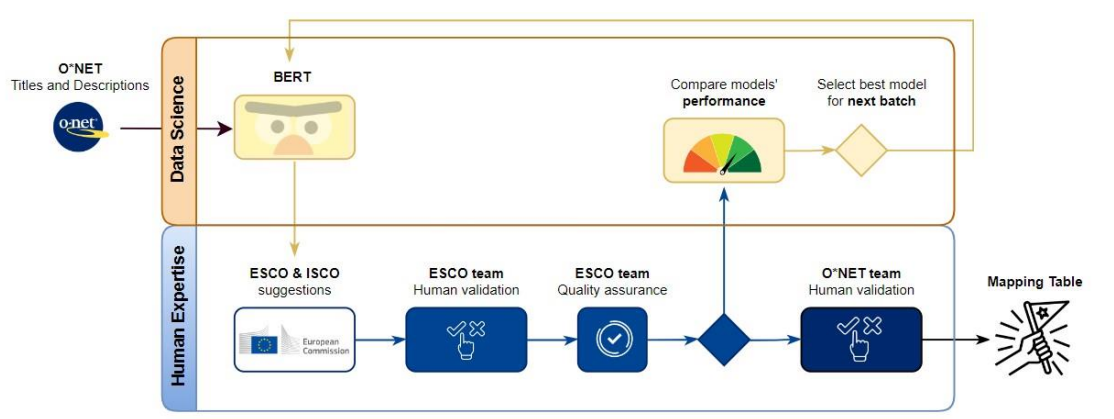
\includegraphics[width=15cm]{figs/crosswalk.png}
    \caption{ESCO-O*NET crosswalk methodology~\cite{esco_onet_crosswalk}}
    \label{fig:crosswalk}
\end{figure}

The European Commission developed AI models (fine-tuned BERT base-uncased) to match \ac{onet} occupations to \ac{esco} occupations based on textual similarity. These models were trained using expert feedback, national taxonomies, qualifications, and job vacancies. The best model suggested ten \ac{esco} occupations for each \ac{onet} occupation, representing the highest semantic similarity. Then, the \ac{esco} team validated these suggestions, distributing the tasks among members and following specific rules to determine the relationship between O*NET-ESCO pairs. The validation process included quality checks and, if necessary, third-party involvement for disagreements. 

This project involved two parallel efforts: iterative improvements by the data science team based on validation feedback and collaboration with the U.S. Department of Labor for further validation and refinement. The final crosswalk table, agreed upon by both teams, is now available on the \ac{esco} Portal.

\section{Large Language Models (LLMs)}
\label{sec:llms}

\ac{llms} consisting of Neural Networks with billions of parameters and trained on vast quantities of unlabeled data (to understand language patterns, grammar and semantics) and labeled data (to guide the model towards more specific tasks)~\cite{lyu2023improving} have significantly impacted the fields of \ac{nlp} and Artificial Intelligence (AI), representing a major transition in how machines understand and generate human language and how they return the information. The history of \ac{llms} is rooted in the development of Machine Learning (ML) and \ac{nlp}, with their emergence being a complete change in the game when it comes to algorithm enhancing, computational power, data availability and data retrieval.

As mentioned, \ac{nlp} has been fundamental to the development and operation of \ac{llms}. Its approach usually involves the execution of a software pipeline with the aim of extracting information from text~\cite{CHIARELLO2021121177}. These approaches have been widely used in different fields, for example, in the analysis of customer reviews, social media usage, patents and, more recently, in the analysis of skill demand and job profiles~\cite{CHIARELLO2021121177, Fareri_2021}.

The field's progression from syntactic analysis to understanding semantics and pragmatics of language has directly influenced the capabilities of these models. \ac{nlp} techniques are crucial in pre-processing data for \ac{llms}, handling tasks like tokenization, part-of-speech tagging, and entity recognition, which are vital for training these models effectively. Furthermore, advances in \ac{nlp} have continually pushed the boundaries of what's possible with \ac{llms}, leading to more sophisticated and context-aware models.

Today, \ac{llms} are an integral part of a wide range of applications. From chatbots and virtual assistants to advanced text generation and translation, they have shown their ability to improve performance on text retrieval tasks through the generation of synthetic training data based on real examples~\cite{clavié2023large}, transforming the way machines interact with human language. 

With the increasing use of \ac{llms}, the concern in developing and optimizing prompts to achieve the best possible answers gave rise to a new discipline, Prompt Engineering~\cite{prompt_engineering}. Prompt engineering is much more than just designing and developing prompts. It gathers a certain set of skills and techniques that enhance the interaction and development with \ac{llms}, allowing for their augmentation with domain knowledge and external tools.

In the context of this work, we will discuss two important techniques of Prompt Engineering, \textbf{Zero-Shot Prompting} and \textbf{Role-Play Prompting}.

In \ac{nlp} and \ac{llms}, Zero-Shot Prompting is understood as providing a prompt to the model that is not part of the training data, but for which the model can provide a desirable result or answer~\cite{zero_few}. This technique relies mainly on the model’s reasoning.

\begin{figure}[H]
    \centering
    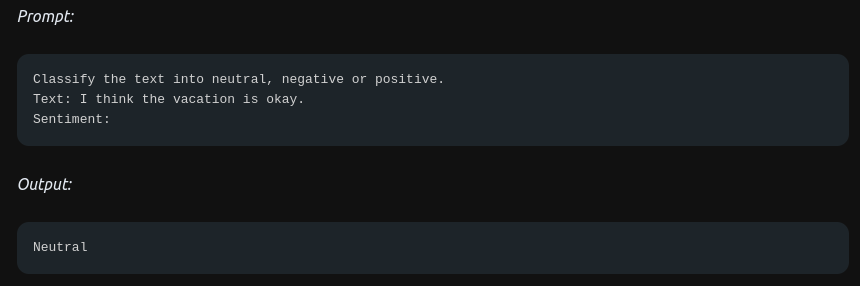
\includegraphics[width=15cm]{figs/zero_shot.png}
    \caption{Example of a Zero-Shot prompt and answer~\cite{zero_shot}}
    \label{fig:zero_shot}
\end{figure}


In Figure \ref{fig:zero_shot} a simple application of \textbf{Zero-Shot Prompting} is represented, where no context or further information is given, just a simple task that tests the model’s reasoning. In the next section, an application of this technique, focused on skills matching, is explored.

Modern \ac{llms}, such as \textit{ChatGPT} and \textit{Google Bard} show an extraordinary capacity for role-playing, being able to not only embody human characters, but also non-human entities, such as the Linux terminal~\cite{kong2023better}. That capacity can be referred to as \textbf{Role-Play Prompting}. This behavior allows the models to simulate complex human-like interactions and perform certain tasks differently, regarding the context prompted and the entity they are embodying. This is a really important feature that can be very useful for this work and will be further discussed in Chapter \ref{chapter:methodology}.

\section{Applying NLP and LLMs to Occupation and Skill Taxonomies}
\label{sec:applying}
As we’ve seen in the previous section, \ac{nlp} and \ac{llms} offer sophisticated tools that can be used to interpret and process text from job descriptions and educational/training offers, helping in mapping their content to \ac{esco} competences, for example.

Therefore, this section will cover various aspects and approaches related to the use of \ac{nlp} and \ac{llms} in the specific context of skill extraction and subsequent alignment with occupational taxonomies, specifically focusing on the matching of these skills to the \ac{esco} framework.


\subsection{Skill-Span Extraction}
\label{sec:skillspan}
The paper~\citetitle{zhang2022skillspan}~\cite{zhang2022skillspan} presents an innovative approach to extract skills from job postings. It roughly consists of a dataset of job postings annotated at the span-level\footnote{A span is a specific, continuous segment of text} for hard and soft skills. Initially, the authors focus on manual annotations by domain experts, to accurately identify specific spans of text that correspond to skills in job postings. This manual annotation is crucial because it will be used to train and fine-tune various BERT models for automatic skill extraction and classification of the manually annotated skill spans. The effectiveness of these models is also explored, highlighting the importance of fine-grained, span-level annotations for a more accurate representation of skills in job postings.

While the final goal of this study is to provide a well-built approach on automated skill extraction, the initial step of dataset creation and annotation relies heavily on human expertise, which is a very lengthy and time-consuming process, especially if we take into account that \ac{esco} contains 13,890 skills. In the following section, a method to fully automate this process is proposed.


\subsection{Zero-Shot Matching}
In~\citetitle{clavié2023large}, the authors explore the application of \ac{llms} in skill matching tasks, particularly mapping job descriptions to \ac{esco} competences. In this approach, a well-thought synthetic data generation is carried out~\cite{clavié2023large}: for each of the 13,890 skills contained in \ac{esco}, they prompted GPT-3.5 to generate forty example sentences that could be used in a job posting in order to refer to the skill. The prompt used for this purpose is provided by the authors in the appendix of the paper.  

Furthermore,~\citeauthor{clavié2023large} propose a two-step process for their skills matching pipeline: initially generating a list of potential matches for a given job description, followed by re-ranking these matches. 
To generate the list of potential matches, the authors use two distinct approaches. The first one relies on simple logistic regression classifiers and the second one is based on cosine similarity between the job description text and the sentences previously generated by GPT-3.5.

In the second phase of the skills matching, \ac{llms} are employed as zero-shot re-rankers (explained in section \ref{sec:llms}~\cite{prompt_engineering}) i.e., without further context, the LLM is prompted to rank the list of potential matches according to their relevance or appropriateness for the job post. 

This approach, requiring no human annotations, significantly outperforms previous methods, highlighting the transformative impact of \ac{llms} in automating and refining the process of mapping complex job descriptions to specific skill sets within a recognized framework, in the case, \ac{esco}.

\begin{figure}[H]
    \centering
    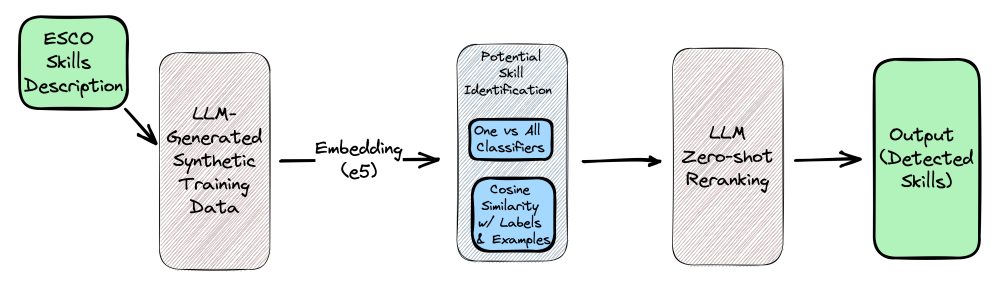
\includegraphics[width=15cm]{figs/zero_shot_process.png}
    \caption{High-level overview of the full Zero-Shot process~\cite{clavié2023large}}
    \label{fig:zero_shot_process}
\end{figure}


\subsection{Distant Supervision}
\label{sec:supervision}
In~\citetitle{zhang2022kompetencer}~\cite{zhang2022kompetencer} and ~\citetitle{decorte2022design}~\cite{decorte2022design} a distinct approach is taken. In these two papers, the authors rely on distant supervision for skill extraction, although with some differences between them. 
“Distant supervision is a technique of labeling data for relation extraction utilizing an existing knowledge database”~\cite{10.1371/journal.pone.0216913}, in this specific context, the database is \ac{esco}.

In~\cite{decorte2022design} the authors use distant supervision to create a training set for skill extraction (Fig. \ref{fig:negative_sampling} - 2). They collect sentences from job vacancies (Fig. \ref{fig:negative_sampling} - 1) that explicitly mention skills of the \ac{esco} taxonomy, a highly precise method that can, however, lead to false negatives. Then, negative sampling strategies are introduced to improve learning (Fig. \ref{fig:negative_sampling} - 3), this consists in “combining ‘positive sentences’ for a given skill (i.e., sentences labeled with that skill during the distant supervision step) with sentences not containing that skill (referred to as ‘negative sentences’)”. Finally, a pre-trained RoBERTa model is used to train binary classifiers for each skill (Fig. \ref{fig:negative_sampling} - 4).

\begin{figure}[H]
    \centering
    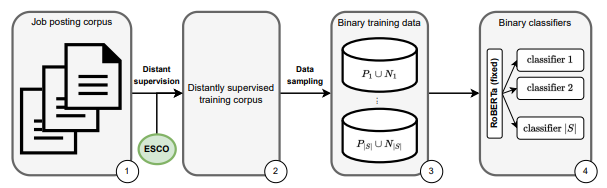
\includegraphics[width=15cm]{figs/negative_sampling.png}
    \caption{Schematic representation of Negative-Sampling processes~\cite{decorte2022design}}
    \label{fig:negative_sampling}
\end{figure}

In~\cite{zhang2022kompetencer}, ~\citeauthor{zhang2022kompetencer} also use distant supervision, in this case, with the \ac{esco} API as reference. The authors annotate a Danish job posting dataset at a span-level, i.e., they identify and label spans within the dataset that correspond to particular skills (following the same logic as explained in the section \ref{sec:skillspan}), while using the \ac{esco} API for distant supervision to obtain fine-grained labels. After that, various BERT models are fine-tuned on the distantly supervised labels and used to classify the spans. Besides that, the authors even presented experiments based on Zero-Shot and Few-Shot Prompting to address the problem of skill extraction.

\begin{figure}[H]
    \centering
    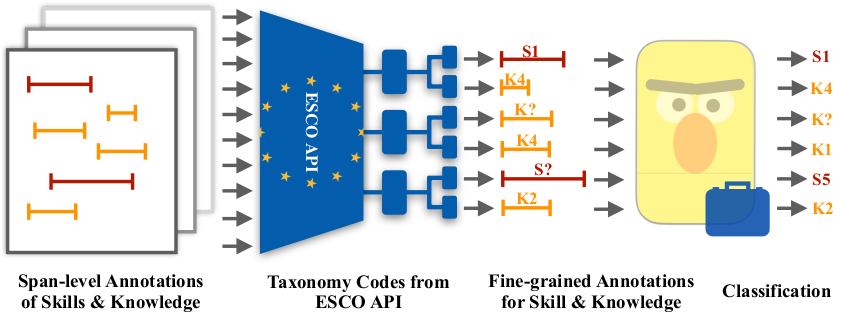
\includegraphics[width=15cm]{figs/kompetencer.png}
    \caption{Pipeline for Fine-grained Danish Skill Classification in Kompetencer~\cite{zhang2022kompetencer}}
    \label{fig:kompetencer}
\end{figure}



For this dissertation work, a mixture of the \textbf{Zero-Shot approach} and the \textbf{Distant Supervision} approach should take place in order to take maximum advantage of both LLM and \ac{esco} API. The data generation method used by~\citeauthor{clavié2023large}~\cite{clavié2023large} could also be adapted for this thesis in order to process all of the \ac{esco} skills, but generating educational offers instead of job postings. However, the other presented approaches will also be taken into account during the implementation of this thesis work, as they provide interesting insights and solutions for different problems.
